%
% CSE Electronic Homework Template
% Last modified 8/23/2018 by Jeremy Buhler

\documentclass[11pt]{article}
\usepackage[left=0.7in,right=0.7in,top=1in,bottom=0.7in]{geometry}
\usepackage{fancyhdr} % for header
\usepackage{graphicx} % for figures
\usepackage{amsmath}  % for extended math markup
\usepackage{amssymb}
\usepackage[bookmarks=false]{hyperref} % for URL embedding
\usepackage[noend]{algpseudocode} % for pseudocode
\usepackage[plain]{algorithm} % float environment for algorithms

%%%%%%%%%%%%%%%%%%%%%%%%%%%%%%%%%%%%%%%%%%%%%%%%%%%%%%%%%%%%%%%%%%%%%%
% STUDENT: modify the following fields to reflect your
% name/ID, the current homework, and the current problem number

% Example: 
%\newcommand{\StudentName}{Jeremy Buhler}
%\newcommand{\StudentID{123456}

\newcommand{\StudentName}{Ming-Che Teng}
\newcommand{\StudentID}{466303}
\newcommand{\HomeworkNumber}{3}

%%%%%%%%%%%%%%%%%%%%%%%%%%%%%%%%%%%%%%%%%%%%%%%%%%%%%%%%%%%%%%%%%%%%%%%%
% You can pretty much leave the stuff up to the next line of %%'s alone.

% create header and footer for every page
\pagestyle{fancy}
\fancyhf{}
\lhead{\textbf{\StudentName}}
\chead{\textbf{\StudentID}}
\rhead{\textbf{Assignment \HomeworkNumber}}
\cfoot{\thepage}

% preferred pseudocode style
\algrenewcommand{\algorithmicprocedure}{}
\algrenewcommand{\algorithmicthen}{}

% ``do { ... } while (cond)''
\algdef{SE}[DOWHILE]{Do}{doWhile}{\algorithmicdo}[1]{\algorithmicwhile\ #1}%

% ``for (x in y ... z)''
\newcommand{\ForRange}[3]{\For{#1 \textbf{in} #2 \ \ldots \ #3}}

% these are common math formatting commands that aren't defined by default
\newcommand{\union}{\cup}
\newcommand{\isect}{\cap}
\newcommand{\ceil}[1]{\ensuremath \left\lceil #1 \right\rceil}
\newcommand{\floor}[1]{\ensuremath \left\lfloor #1 \right\rfloor}
\newcommand*{\Perm}[2]{{}^{#1}\!P_{#2}}%
\newcommand*{\Comb}[2]{{}^{#1}C_{#2}}%
\newcommand*{\Int}{\int\limits}
\usepackage{listings}
\usepackage{color}


\definecolor{dkgreen}{rgb}{0,0.6,0}
\definecolor{gray}{rgb}{0.5,0.5,0.5}
\definecolor{mauve}{rgb}{0.58,0,0.82}
\lstset{frame=tb,
  language=Java,
  aboveskip=3mm,
  belowskip=3mm,
  showstringspaces=false,
  columns=flexible,
  basicstyle={\small\ttfamily},
  numbers=none,
  numberstyle=\tiny\color{gray},
  keywordstyle=\color{blue},
  commentstyle=\color{dkgreen},
  stringstyle=\color{mauve},
  breaklines=true,
  breakatwhitespace=true,
  tabsize=3
}

%%%%%%%%%%%%%%%%%%%%%%%%%%%%%%%%%%%%%%%%%%%%%%%%%%%%%%%%%%%%%%%%%%%%%%

\begin{document}
\subsection * {Problems}

\begin{enumerate}

\item [\textbf{1.}]  

\textbf{LFD Problem 4.4 MATLAB implementation}

(a)

\begin{equation}
\begin{aligned}
E_{a,x}[f^2] =& E_{a,x}[(a_0L_0(x) + a_1L_1(x) + ... + a_{Qf}L_{Qf}(x))^2]\\
\because & \int_{-1}^{1} L_k(x)L_l(x)dx 
= \begin{cases}
0 & \text{$l \neq k$}\\
\frac{2}{2k+1} & \text{$l = k$}
\end{cases}
\text{ and } E_x(f(x)) = \int_{a}^{b} P(x)f(x)dx\\
=& E_{a,x} [f^2] = E_a[\int_{-1}^{1}(a_0L_0(x) + a_1L_1(x) + ... + a_{Qf}L_{Qf}(x))^2]\\
=& E_a[\sum_{q=0}^{Qf}\frac{a_q^2}{2q+1}]\\
=& E[a_0^2] + \frac{1}{3}E[a_1^2] + ... + \frac{1}{2Q_f+1}E[a_{Qf}^2]\\
\because & \sigma^2 = 1, \text{ then } E[a_i^2] = \sigma^2 - (E[a_i]^2)^2 = 1 - 0 = 1, \text{ for } i = 1, 2, ..., Qf\\
\therefore & E[a_0^2] + \frac{1}{3}E[a_1^2] + ... + \frac{1}{2Q_f+1}E[a_{Qf}^2] \\
=& 1 + \frac{1}{3} + \frac{1}{5} + ... + \frac{1}{2Q_f+1} = \sum_{q=0}^{Q_f} \frac{1}{2q+1}\\
=& E_{a,x}[f^2] = \sum_{q=0}^{Q_f} \frac{1}{2q+1}
\end{aligned}
\end{equation}

Let the result to 1, the term can be normalized when each $a_i$, for $ i = 1, 2, ..., Q_f$, is divided by the normalizer $\sqrt{\sum_{q=0}^{Q_f}\frac{1}{2q+1}}$ , that is, $\tilde{a} = \frac{a_i}{\sqrt{\sum_{q=0}^{Q_f}\frac{1}{2q+1}}}$

The reason to normalize $f$ is that normalizing $E_{a,x}[f^2] = 1$ let the noise level $\sigma^2$ automatically calibrated to the signal level.

(b)

To obtain $g_2$ and $g_10$, we transform the original data $x \in X$ with a second order transformation and 10th order transformation. Then, we can find the best linear fit for the data in $Z_2$ and $Z_{10}$.

The implementation is as follows,
\begin{lstlisting}
z_train_2 = L(x_train,2)
z_train_10 = L(x_train,10)
w2 = glmfit(z_train_2, y_train, 'normal', 'constant', 'off')
w10 = glmfit(z_train_10, y_train, 'normal', 'constant', 'off')
g2 = computeLegPoly(x_test, 2) * w2
g10 = computeLegPoly(x_text, 10) * w10
\end{lstlisting}



(c)

To compute analytically $E_{out}$ for a given $g_{10}$, 

\begin{equation}
\begin{aligned}
E_{out} =& E_{x,y}[(g_{10}(x) - y)^2]\\
=& E_{x,\epsilon}[(g_{10}(x) - (f(x) + \sigma\epsilon))^2]\\
=& E_{x,\epsilon}[(g_{10}(x) - f(x))^2 -2(g_{10}(x) - f(x))\sigma\epsilon + (\sigma\epsilon)^2]\\
=& E_{x,\epsilon}[(\sum_{i=0}^{10}w_iL_i(x) - \sum_{j=0}^{Q_f}a_jL_j(x))^2 - 2(\sum_{i=0}^{10}w_iL_i(x) - \sum_{j=0}^{Q_f}a_jL_j(x))\sigma\epsilon + (\sigma\epsilon)^2]\\
\because & E_{\epsilon}[\epsilon] = 0 \rightarrow E_{x,\epsilon}[- 2(\sum_{i=0}^{10}w_iL_i(x) - \sum_{j=0}^{Q_f}a_jL_j(x))\sigma\epsilon] = 0\\
\because & E_{\epsilon}[\epsilon^2] = 1 \rightarrow E_{x,\epsilon} [(\sigma\epsilon)^2] = \sigma^2\\
E_{out} =  &E_{x,\epsilon}[(\sum_{i=0}^{10}w_iL_i(x) + \sum_{j=0}^{Q_f}a_jL_j(x))^2 + \sigma^2]\\
=& E_{x,\epsilon} [(\sum_{i=0}^{10}w_iL_i(x))^2 - 2\sum_{j=0}^{min(10,Q_f)}(w_ja_jL_j(x))^2 + \sum_{k=0}^{Q_f}(a_kL_k(x))^2 + \sigma^2]\\
=& E_{\epsilon} [\sum_{i=0}^{10}\frac{w_i^2}{2i+1} - 2\sum_{j=0}^{min(10,Q_f)}\frac{w_ja_j}{2j+1} + \sum_{k=0}^{Q_f} \frac{a_k^2}{2k+1} + \sigma^2]\\
=& \sum_{i=0}^{10}\frac{w_i^2}{2i+1} \textendash -2\sum_{j=0}^{min(10,Q_f)}\frac{w_ja_j}{2j+1} + \sum_{k=0}^{Q_f} \frac{a_k^2}{2k+1} + \sigma^2
\end{aligned}
\end{equation}

(d)

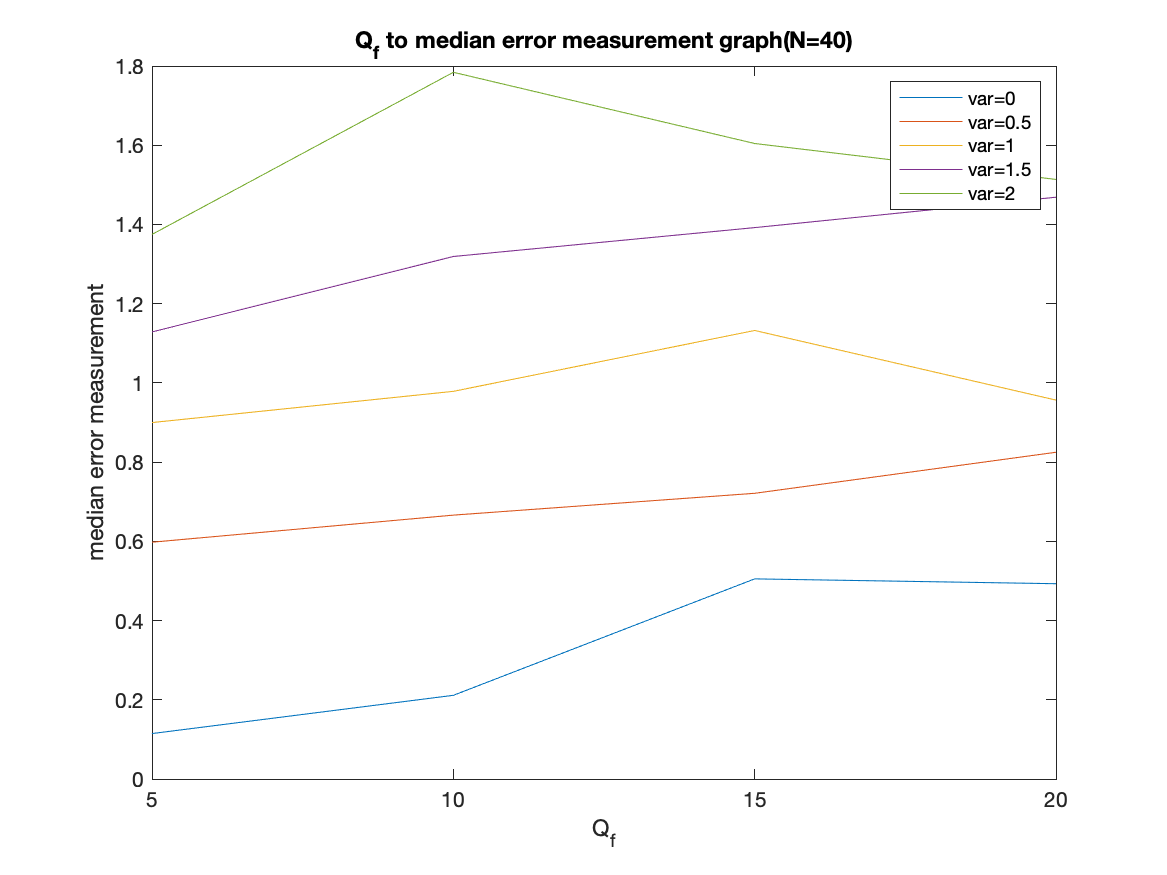
\includegraphics[scale = 0.4]{/Users/alexteng/Desktop/CSE417/h4_1.png}
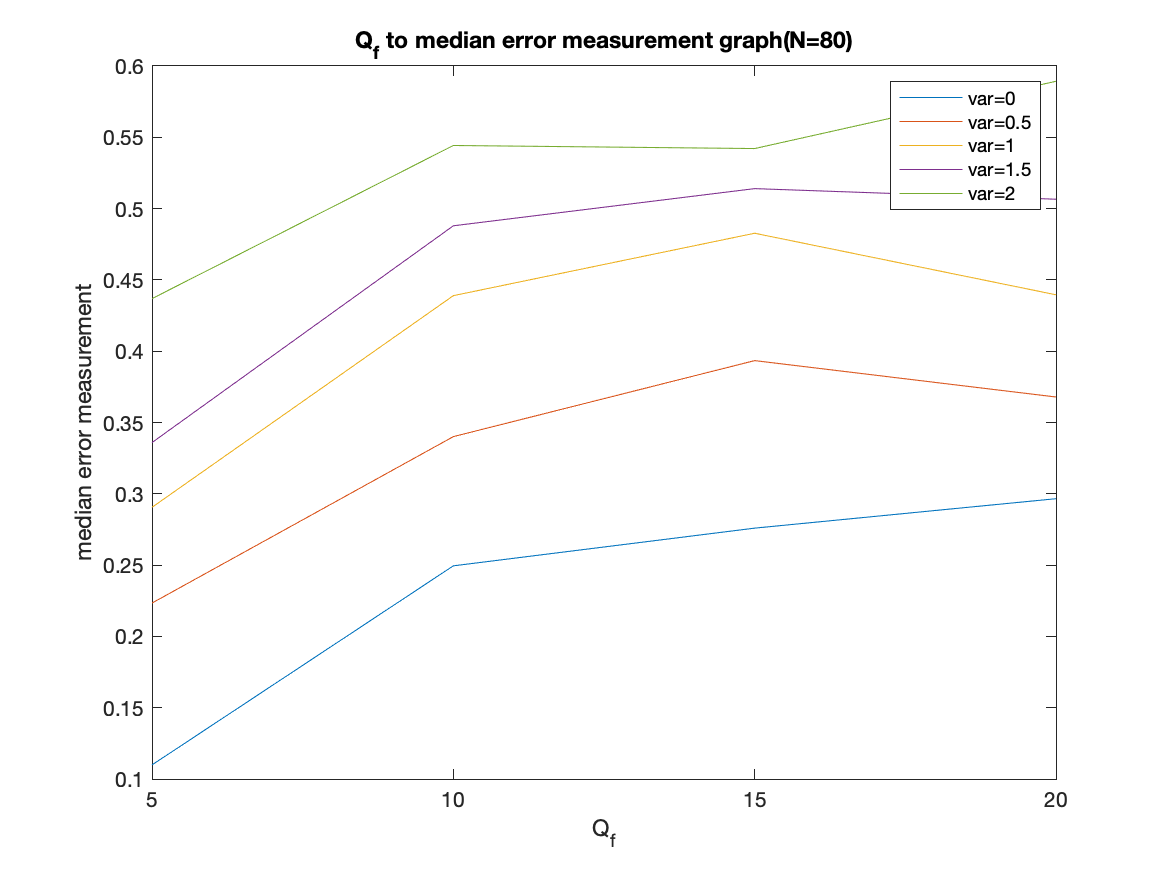
\includegraphics[scale = 0.4]{/Users/alexteng/Desktop/CSE417/h4_2.png}

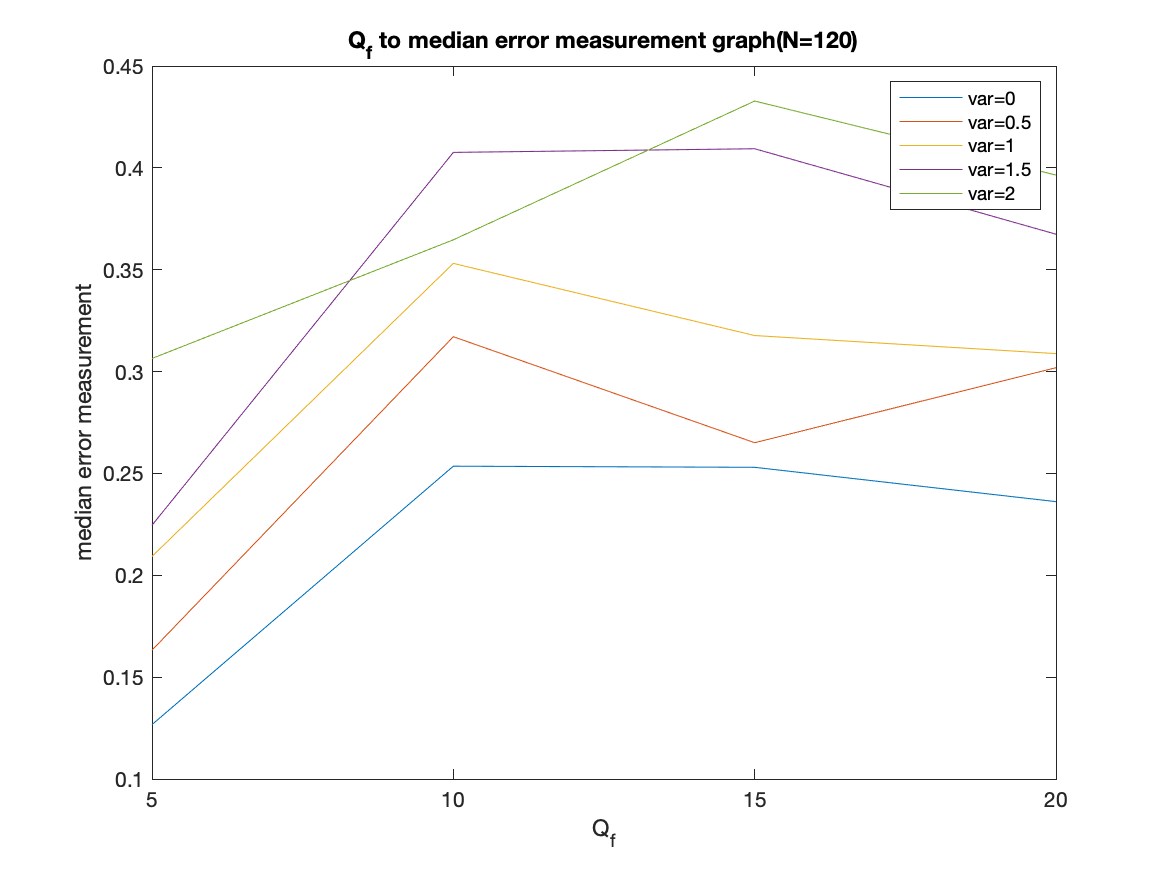
\includegraphics[scale = 0.4]{/Users/alexteng/Desktop/CSE417/h4_3.png}
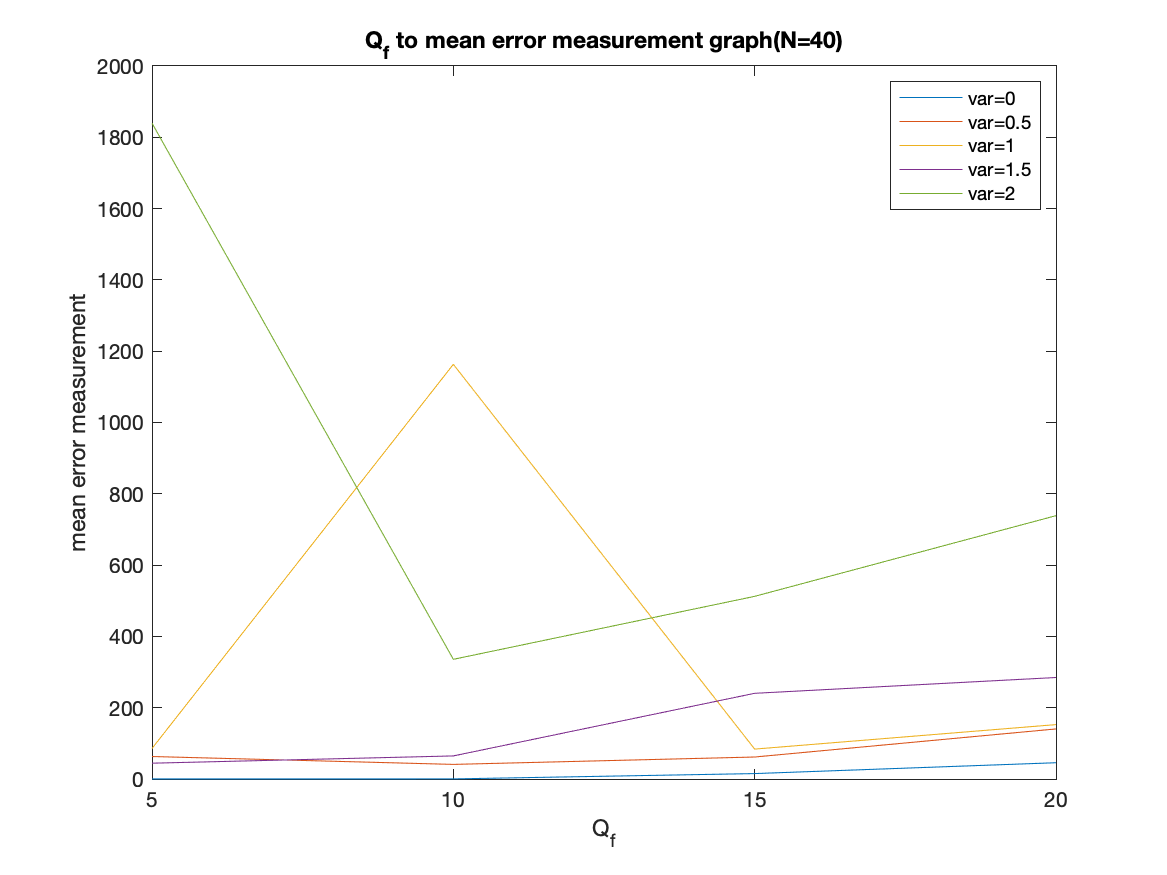
\includegraphics[scale = 0.4]{/Users/alexteng/Desktop/CSE417/h4_4.png}

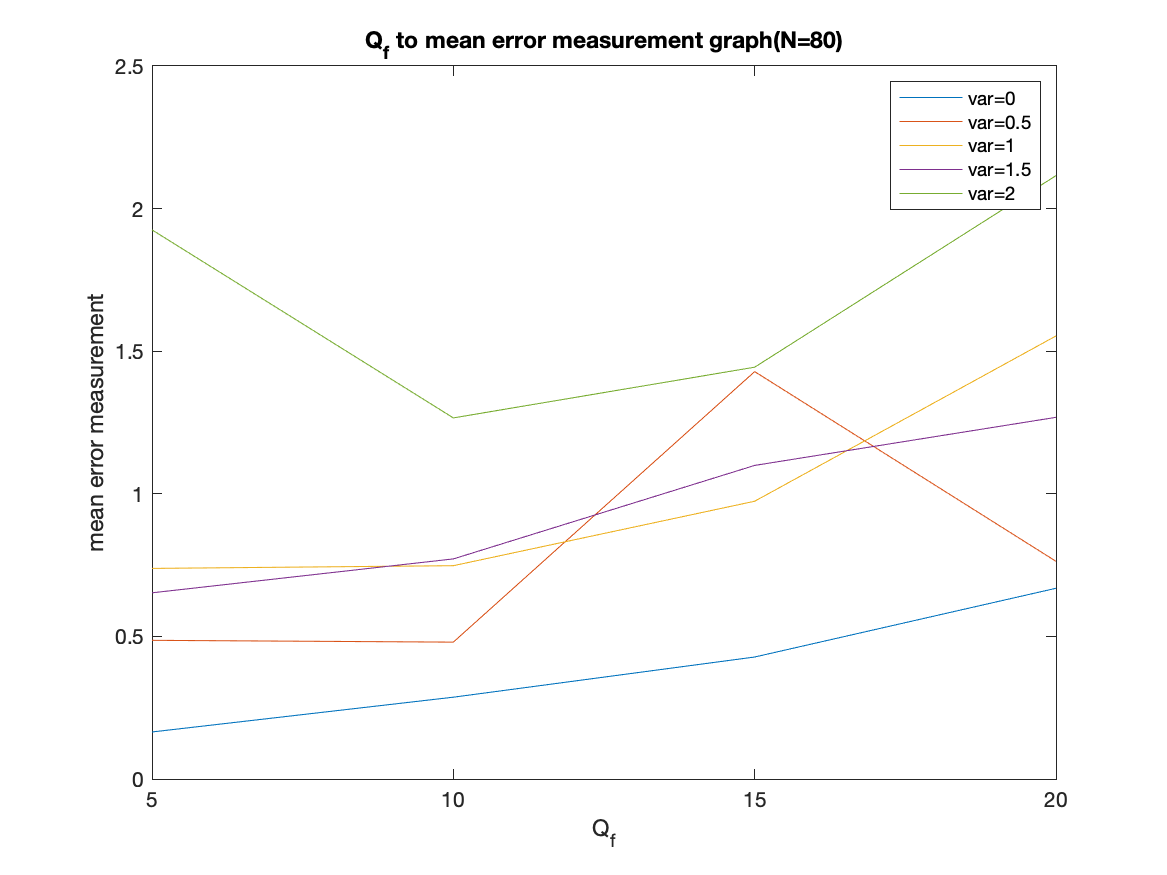
\includegraphics[scale = 0.4]{/Users/alexteng/Desktop/CSE417/h4_5.png}
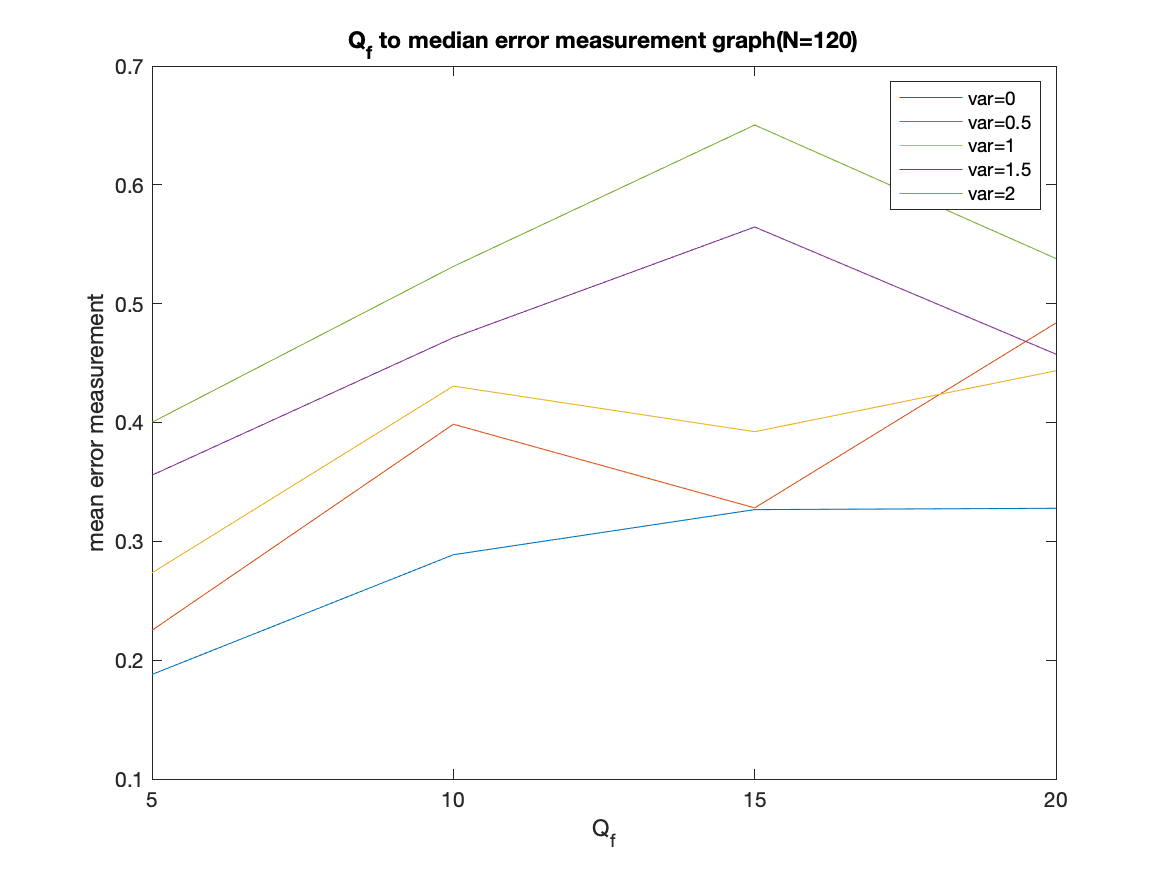
\includegraphics[scale = 0.4]{/Users/alexteng/Desktop/CSE417/h4_6.png}

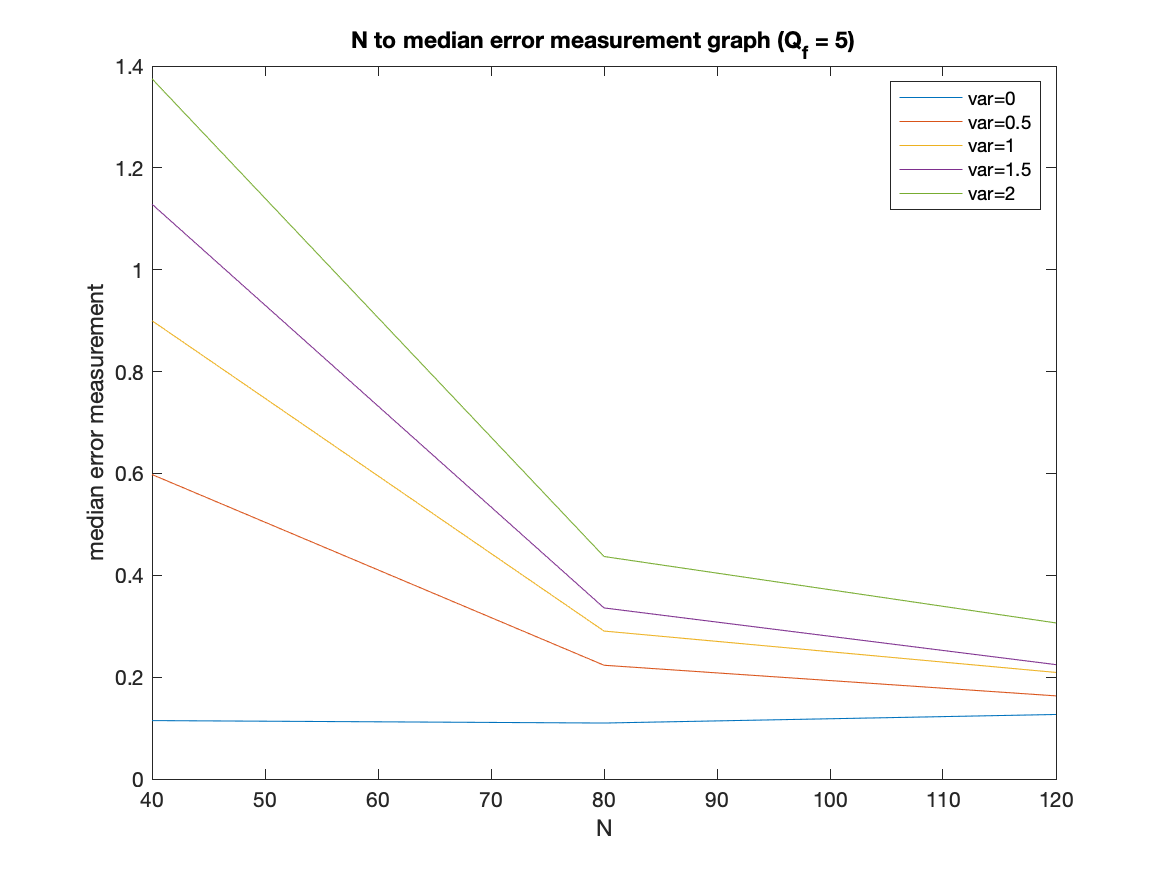
\includegraphics[scale = 0.4]{/Users/alexteng/Desktop/CSE417/h4_7.png}
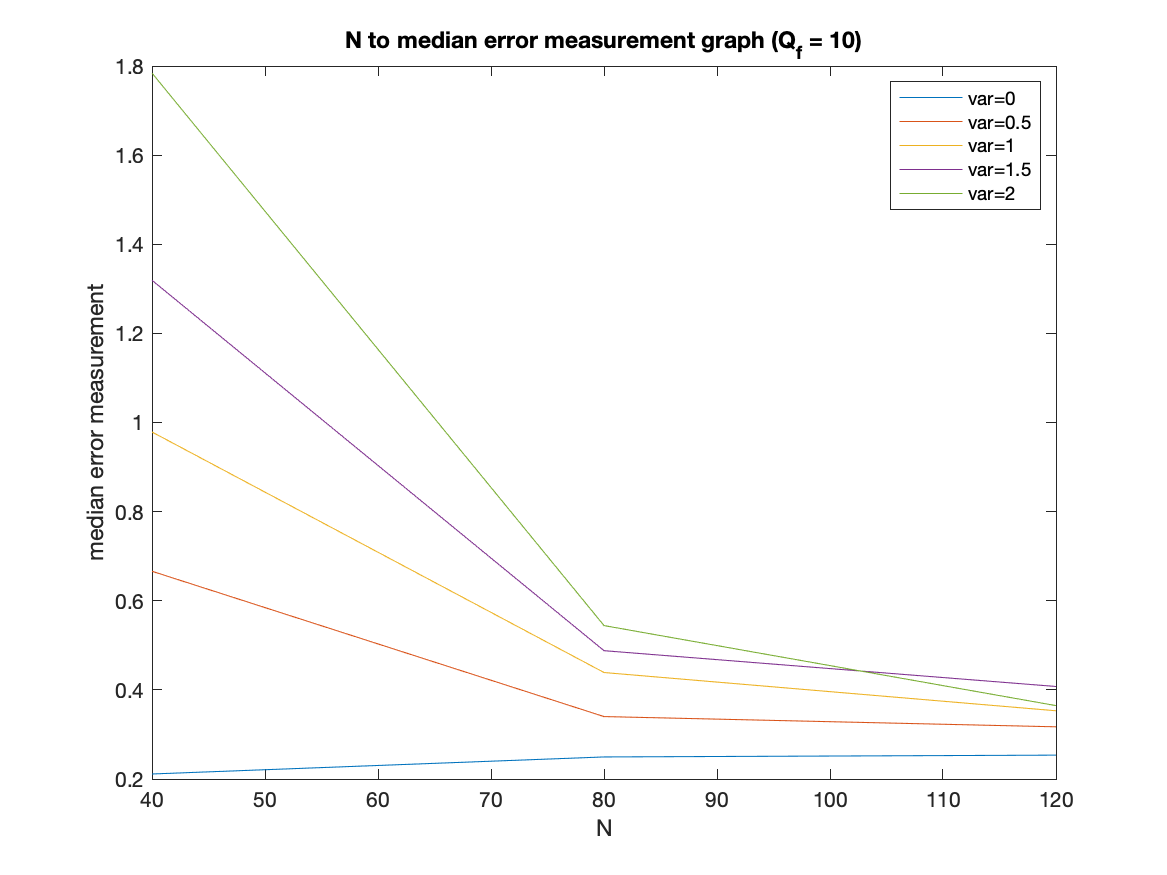
\includegraphics[scale = 0.4]{/Users/alexteng/Desktop/CSE417/h4_8.png}

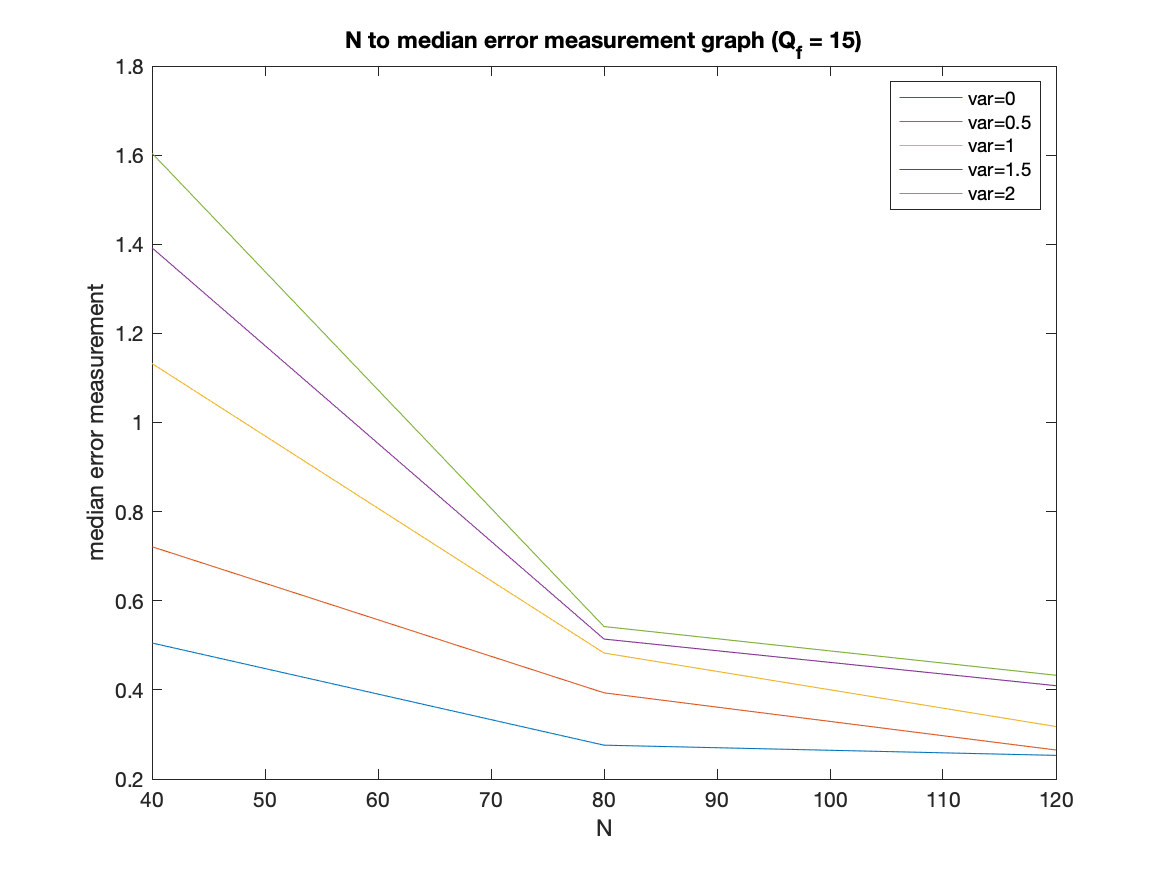
\includegraphics[scale = 0.4]{/Users/alexteng/Desktop/CSE417/h4_9.png}
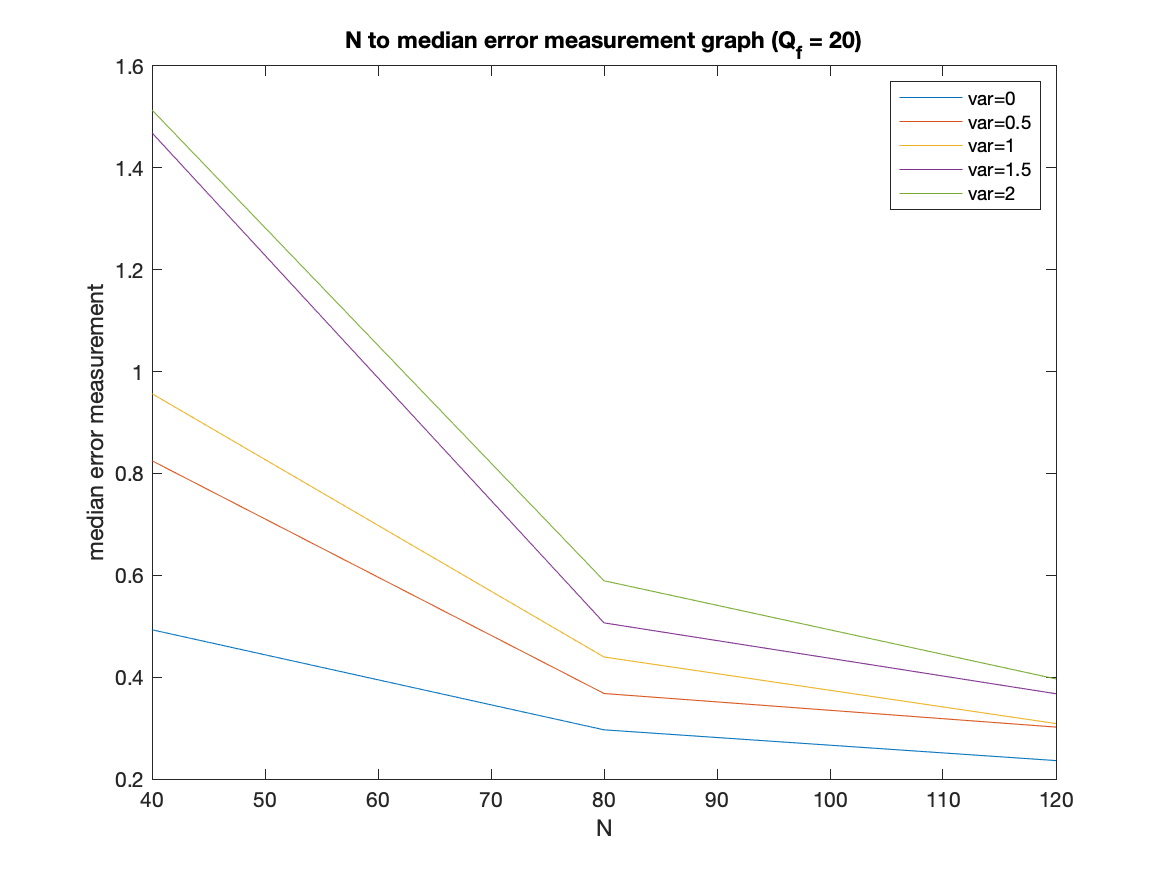
\includegraphics[scale = 0.4]{/Users/alexteng/Desktop/CSE417/h4_10.png}

The above are the results based on different size of training set, variance, and $Q_f$, and using median and mean to measure the out-of sample error.

The explanations are as follows,

First, serious overfitting happens when using mean error measurement, model complexity is large, number of training data is small, and nose coefficient is large. 

Especially, error measurements grows positively larger when model complexity and N goes larger. 

Given sufficiently large N, say N = 80 or 120, the difference complex model and simple model grows larger when model complexity, $Q_f$, goes up.

Without stochastic noise, $\sigma$, error measurement is larger than those in the same N and $Q_f$ with stochastic noise.

Summing up, 

overfitting goes up when stochastic noise, $\sigma$, goes up, especially when N is small.

overfitting goes up when model complexity, $Q_f$, goes up.

overfitting goes down when number of training data, N, goes up.

Comments:

The result using mean error measurement is very volatile as it counts very extreme case into average, for example, extreme positive or negative $\epsilon$ or $\sigma$.

Using median error measurement can give us more consistent result due to picking median value.

\pagebreak

\begin{table}[h!]
  \begin{center}
    \caption{Results Table with Different $Q_f$, $N$, Variance, and Method of Measurement}
    \label{tab:table1}
    \begin{tabular}{l|c|c|c|c|c|c|c|r}
    \hline
    \multicolumn{4}{|c|}{Mean error measurement} & \multicolumn{4}{|c|}{Median error measurement}\\
      \hline
      \text{$var=0$} & \text{$N=40$} & \text{$N=80$} & \text{$N=120$} & \text{$var=0$} & \text{$N=40$} & \text{$N=80$} & \text{$N=120$}\\
      \hline
      \text{$Q_f = 5$} &  \text{0.1564} & \text{0.1649} & \text{0.1880} & \text{$Q_f =5$ } & \text{0.1147} & \text{0.1099}& \text{0.1267} \\
      \hline
      \text{$Q_f = 10$} & \text{0.2369} & \text{0.2868} & \text{0.2887} & \text{$Q_f=10$} & \text{0.2112}& \text{0.2495}& \text{0.2536}\\
      \hline
      \text{$Q_f = 15$} & \text{15.1976} & \text{0.4277} & \text{0.3267} & \text{$Q_f=15$} & \text{0.5052}& \text{0.2759}& \text{0.2530}\\
      \hline
      \text{$Q_f = 20$} & \text{45.6467} & \text{0.6688} & \text{0.3278} & \text{$Q_f=20$} & \text{0.4930}& \text{0.2966}& \text{0.2362}\\
            \hline
      \text{$var=0.5$} & \text{$N=40$} & \text{$N=80$} & \text{$N=120$} & \text{$var=0.5$} & \text{$N=40$} & \text{$N=80$} & \text{$N=120$}\\
      \hline
      \text{$Q_f = 5$} &  \text{63.0766} & \text{0.4862} & \text{0.2251} & \text{$Q_f =5$ } & \text{0.5978} & \text{0.2234}& \text{0.1632} \\
      \hline
      \text{$Q_f = 10$} & \text{40.9573} & \text{0.4799} & \text{0.3985} & \text{$Q_f=10$} & \text{0.6661}& \text{0.3401}& \text{0.3171}\\
      \hline
      \text{$Q_f = 15$} & \text{61.6690} & \text{1.4284} & \text{0.3281} & \text{$Q_f=15$} & \text{0.7213}& \text{0.3934}& \text{0.2651}\\
      \hline
      \text{$Q_f = 20$} & \text{140.4305} & \text{0.7632} & \text{0.4843} & \text{$Q_f=20$} & \text{0.8249}& \text{0.3679}& \text{0.3019}\\
       \hline
      \text{$var=1$} & \text{$N=40$} & \text{$N=80$} & \text{$N=120$} & \text{$var=1$} & \text{$N=40$} & \text{$N=80$} & \text{$N=120$}\\
      \hline
      \text{$Q_f = 5$} &  \text{85.6} & \text{0.7384} & \text{0.2735} & \text{$Q_f =5$ } & \text{0.8998} & \text{0.2905}& \text{0.2092} \\
      \hline
      \text{$Q_f = 10$} & \text{1163} & \text{0.7479} & \text{0.4306} & \text{$Q_f=10$} & \text{0.9787}& \text{0.4389}& \text{0.3531}\\
      \hline
      \text{$Q_f = 15$} & \text{83.87} & \text{0.9739} & \text{0.3923} & \text{$Q_f=15$} & \text{1.1324}& \text{0.4827}& \text{0.3177}\\
      \hline
      \text{$Q_f = 20$} & \text{152.6} & \text{1.554} & \text{0.4435} & \text{$Q_f=20$} & \text{0.9565}& \text{0.4396}& \text{0.3088}\\
       \hline
      \text{$var=1.5$} & \text{$N=40$} & \text{$N=80$} & \text{$N=120$} & \text{$var=1.5$} & \text{$N=40$} & \text{$N=80$} & \text{$N=120$}\\
      \hline
      \text{$Q_f = 5$} &  \text{44.32} & \text{0.6528} & \text{0.3557} & \text{$Q_f =5$ } & \text{1.1287} & \text{0.3359}& \text{0.2246} \\
      \hline
      \text{$Q_f = 10$} & \text{64.73} & \text{0.7717} & \text{0.4714} & \text{$Q_f=10$} & \text{1.3191}& \text{0.4879}& \text{0.4076}\\
      \hline
      \text{$Q_f = 15$} & \text{240.4} & \text{1.1} & \text{0.5645} & \text{$Q_f=15$} & \text{1.3920}& \text{0.5140}& \text{0.4094}\\
      \hline
      \text{$Q_f = 20$} & \text{284.7} & \text{1.268} & \text{0.4575} & \text{$Q_f=20$} & \text{1.4687}& \text{0.5066}& \text{0.3674}\\
       \hline
      \text{$var=2$} & \text{$N=40$} & \text{$N=80$} & \text{$N=120$} & \text{$var=2$} & \text{$N=40$} & \text{$N=80$} & \text{$N=120$}\\
      \hline
      \text{$Q_f = 5$} &  \text{1840} & \text{1.925} & \text{0.4002} & \text{$Q_f =5$ } & \text{1.3748} & \text{0.4369}& \text{0.3064} \\
      \hline
      \text{$Q_f = 10$} & \text{335.7} & \text{1.266} & \text{0.5315} & \text{$Q_f=10$} & \text{1.7841}& \text{0.5443}& \text{0.3647}\\
      \hline
      \text{$Q_f = 15$} & \text{512.3} & \text{1.444} & \text{0.6503} & \text{$Q_f=15$} & \text{1.6043}& \text{0.5421}& \text{0.4328}\\
      \hline
      \text{$Q_f = 20$} & \text{738.7} & \text{2.116} & \text{0.538} & \text{$Q_f=20$} & \text{1.5136}& \text{0.5893}& \text{0.3965}\\


    \end{tabular}
  \end{center}
\end{table}
\end{enumerate}

\pagebreak

\subsection*{Problems}
\begin{enumerate}

\item[\textbf{2.}]

\textbf{LFD Exercise 4.5}

(a)

A softer order constraint is $\sum_{q=0}^{Q}w_q^2 \leq C$, which is stated in the textbook.
As the Tikhonov regularizer is a more general constraint regularizer, we can consider it as an identity matrix, that is $I$ and that would give as an equation that is exactly the same as $\sum_{q=0}^{Q}w_q^2 \leq C$ in the textbook.

\begin{equation}
w^TI^TIw = 
\begin{pmatrix}
	w_0 & w_1 & w_2 & ...\\
\end{pmatrix}
\begin{pmatrix}
	1 & 0 & 0 & ... \\
	0 & 1 & 0 & ... \\
	0 & 0 & 1 & ... \\
	. & . & . & ...\\
\end{pmatrix}
\begin{pmatrix}
	1 & 0 & 0 & ... \\
	0 & 1 & 0 & ... \\
	0 & 0 & 1 & ... \\
	. & . & . & ...\\
\end{pmatrix}
\begin{pmatrix}
	w_0 \\
	w_1\\
	w_2\\
	.\\
	.\\
	.\\
\end{pmatrix}
= \sum_{q=0}^{Q}w_q^2
\end{equation}

(b)

In order to get the $(\sum_{q=0}^{Q}w_q)^2 \leq C$, the translation of the equation is that summing all the element in the weight vector and then take the square of it, the result is required to less than or equal to $C$. To obtain this result, Tikhonov regularizer should be as follows,

\begin{equation}
w^T\Gamma^T\Gamma w = 
\begin{pmatrix}
	w_0 & w_1 & w_2 & ...\\
\end{pmatrix}
\begin{pmatrix}
	1 & 0 & 0 & ... \\
	1 & 0 & 0 & ... \\
	1 & 0 & 0 & ... \\
	. & . & . & ...\\
\end{pmatrix}
\begin{pmatrix}
	1 & 1 & 1& ... \\
	0 & 0 & 0 & ... \\
	0 & 0 & 0 & ... \\
	. & . & . & ...\\
\end{pmatrix}
\begin{pmatrix}
	w_0 \\
	w_1\\
	w_2\\
	.\\
	.\\
	.\\
\end{pmatrix}
= (\sum_{q=0}^{Q}w_q)^2
\end{equation}

In the equation above, $\Gamma$ should be a matrix with the first element in all columns are all 1, and the result would be $(\sum_{q=0}^{Q}w_q)^2$




\end{enumerate}

\pagebreak

\subsection*{Problems}
\begin{enumerate}
\item[\textbf{3.}]

\textbf{LFD Problem 4.8}

First, $E_{aug}(w) = E_{in} + \lambda w^Tw$, so the gradient is $$ \triangledown E_{aug}(w) = \triangledown E_{in}(w) + 2\lambda w$$

so the gradient descent update becomes

$$w(t+1) \leftarrow w(t) - \eta \triangledown E_{aug}(w(t)) = (1 - 2 \eta \lambda)w(t) - \eta \triangledown E_{in}(w(t))$$

\end{enumerate}

\pagebreak

\subsection*{Problems}
\begin{enumerate}

\item[\textbf{4.}]

\textbf{LFD Problem 4.25}

(a)

No, in this cases, since we will get different size of validation set $K_m$ there are no guarantees that we can get the VC-bound we obtained when using the same validation set for all models. 

(b)

As explained in the theory, since the validation model $H_{val}$ was obtained before looking at the data in the validation set, the process of model selection is equivalent to learning a hypothesis from $H_{val}$ using the data in $D_{val}$. In this case, we can apply the VC-bound for finite hypothesis sets.

(c)

We've already known from the Hoeffding inequality and from the part (b) that for each $m = 1, ..., M$,
$$P[E_{out}(m) - E_{val}(m) > \epsilon] \leq e^{-\epsilon^2K_m}$$

for all $\epsilon$ > 0. And using the union bound method, we can get, 

$$P[E_{out}(m^*) - E_{val}(m^*) > \epsilon] \leq P[E_{out}(1) - E_{val}(1) > \epsilon] + ... + P[E_{out}(M) - E_{val}(M) > \epsilon] \leq \sum_{m=1}^{M}e^{-\epsilon^2K_m}$$

Now, we let $k(\epsilon)= -\frac{1}{2\epsilon^2}\ln(\frac{1}{M}\sum_{m=1}^{M}e^{-2\epsilon^2K_m})$, we can get the following, 

$$Me^{-2\epsilon^2k(\epsilon)} = Me^{\ln(\frac{1}{M}\sum_{m=1}^{M}e^{-2\epsilon^2K_m})} = \sum_{m=1}^{M}e^{-2\epsilon^2K_m}$$

Finally we obtain, $$P[E_{out}(m^*) > E_{val}(m^*) + \epsilon] \leq Me^{-2\epsilon^2k(\epsilon)}$$

Moreover, we may note that $k(\epsilon) \geq 0$ since $-2\epsilon^2K_m \leq 0$, this implies that $e^{-2\epsilon^2K_m}\leq 1$, and so $\frac{1}{M}\sum_{m=1}^{M}e^{-2\epsilon^2K_m}\leq 1$ and finally $k(\epsilon)\geq 0$




\end{enumerate}
\pagebreak
\subsection*{Problems}
\begin{enumerate}

\item[\textbf{5.}]

\textbf{LFD Problem 5.4}

(a)

The problem here is that we need $N=12500$ days (50 years) of data. Although we opted to fix the $M=500$, there's a data snooping involved in this choice since these 500 stocks were also selected beforehand, by the definition of the S\&P 500, which is looking at the whole data set, then selected the largest companies stock to form the portfolio. Moreover, for many of the 50000 stocks we do not have the full 12500 days of data but much less in many circumstances.

As stated above, the correct M should be $M=50000$, the number of stocks that has been traded over the last 50 years. In this conditions, we get $$P[E_{in} - E_{out} > 0.02] \leq 2 \cdot 50000 \cdot e^{-2\cdot 12500 \cdot 0.02^2} \approx 4.53999$$



(b)

As we elaborated in part(a), we cannot conclude with any certainty that buying and holding stocks is a good strategy since we only based on 500 stocks that were selected beforehand. The issue here is called data snooping.

What we would be able to say something about the performance of buy and hold trading is if we considered all 50000 stocks that are currently trading in the market, not just the 500 largest companies selected beforehand by evaluating the company's value.






\end{enumerate}
\pagebreak


\subsection*{Collaboration Statement}

I didn't collaborate with anyone in this assignment.
\end{document}